\documentclass[final]{beamer}
\mode<presentation>

% Change colours on line 3 by setting \usetheme[<id>]{HYposter}.
% The different ids are:
%  maa: Faculty of Agriculture and Forestry 
%  hum: Faculty of Arts 
%  kay: Faculty of Behavioural Sciences 
%  bio: Faculty of Biological and Environmental Sciences 
%  oik: Faculty of Law 
%  med: Faculty of Medicine 
%  far: Faculty of Pharmacy 
%  mat: Faculty of Science 
%  val: Faculty of Social Sciences 
%  teo: Faculty of Theology 
%  ell: Faculty of Veterinary Medicine 
%  soc: Swedish School of Social Science 
%  kir: University of Helsinki Library
%  avo: Open University
%  ale: Aleksanteri Institute
%  neu: Neuroscience Institute
%  biot: Bioscience Institute
%  atk: Computer centre
%  rur: Ruralia Institute
%  koe: Laboratory animal centre
%  kol: Collegium for Advanced Studies
%  til: Center for Properties and Facilities
%  pal: Palmenia
%  kie: Language centre
% Without options a black theme without faculty name will be used.

\usepackage[english]{babel}
\usepackage[T1]{fontenc}
\usepackage[utf8]{inputenc}
\usepackage{lmodern}
\usepackage{exscale}
\usepackage{amsmath,amsthm, amssymb, latexsym}
\usepackage{algorithm}
\usepackage{algpseudocode}

\usepackage[orientation=portrait,size=a0,scale=1.4]{beamerposter}
\usetheme[mat, threecolumn]{HYposter}

% Set up the title and author info
\titlestart{Aho-Corasick and Rabin-Karp}
\titleend{in Multiple Pattern String Matching}
\author{Aleksi Hartikainen and Jussi Kokkala}
\leftcorner{}

\begin{document}
\begin{poster}

\newcolumn

%\section{\LaTeX~posters made easier}
Multiple pattern string matching is ...

Aho --

\section{Rabin-Karp}
      Rabin-Karp uses hashing to find fixed length patterns in a text. The hashing function used is a rolling hash, meaning that the hash of $T[2\;..\;N+1]$ can be calculated from the hash of $T[1..N]$ in constant time. Rabin-Karp in single pattern matching is shown in algorithm \ref{alg:rk_single}.

\begin{algorithm} [H]
\small
\caption{Single pattern Rabin-Karp}
\label{alg:rk_single}

\begin{algorithmic}[1]
\Require{pattern P of length M, text T of length N}

\State $pattern\_hash \gets \text{hash(pattern)}$
\State $text\_hash \gets \text{hash(T[1\;..\;M])}$
\For {$i \gets M \to N$}
    \If{$ i > M$}
        \State  $text\_hash \gets \text{rolling\_hash(text\_hash,T[i-M],T[i])}$
    \EndIf
    \If{$pattern\_hash = text\_hash $}
        \If{$T[i-M+1\;..\;i] = P$}
            \State $\text{enqueue(matches,i-M+1)}$
        \EndIf
    \EndIf
\EndFor
\end{algorithmic}
\end{algorithm}

If the pattern length is fixed, multiple pattern Rabin-Karp can be modified from algorithm \ref{alg:rk_single} by storing all pattern hashes in a hash table and checking every text position against all patterns in the hash table at index $text\_hash$.

If the pattern length is not fixed, it is possible to use fixed length Rabin-Karp separately for each pattern length. Another solution is to use the length $L$ of the shortest pattern, and calculate hashes only up to the $L$th character of each pattern. As this increases the number of false alarms, in practice it is often better to combine these methods and divide the patterns into several groups of similar lengths.

For $P$ patterns of combined length $M$  and a text of length $N$, the average running time of Rabin-Karp is $O(N+M)$ in space $O(P)$.


\section{Aho-Corasick}

Aho-Corasick constructs an automaton (Figure \ref{fig:ac_machine}) which is then computed on the text.
States of this automaton are the nodes of a trie of all patterns strings.
Additionally there are failure links for each state (Dotted edges in figure~\ref{fig:ac_machine}).
, which are followed until matching transition is found. From the root state all failing symbols
have self-transitions.

%Running time of the algorithm is linear in the length of text. Each failure link goes towards the root, so in total we can't use more failure
%links than we do transitions.
%Additional ``back'' state is added to the automaton to make root node behave similarly to all other nodes. 

The failure links are computed using algorithm~\ref{alg:ac_fail}.
Pattern links (shown green in figure~\ref{fig:ac_machine}) are added to each
matching state and from each pattern $s$ there is a link to the longest pattern which
is a suffix of $s$.
Using these links we can easily list all matching patterns for
any state.
\newcolumn

Construction algorithm has time complexity $O(M)$. Total time complexity is $O(N+M)$.

Main disadvantage of Aho-Corasick algorithm is the $O(M)$ space needed to store the automaton.
Our implementation uses $8M+O(P)$ bytes of memory.

\vspace{5mm}

\begin{algorithm} [H]
\small
\caption{Algorithm for computing failure links}
\label{alg:ac_fail}

\begin{algorithmic}[1]
\Require{Trie of patterns}
\Ensure{Failure links for all nodes}
\State $ \text{fail}(\text{root}) \gets \text{fail}$
\State $Q \gets Queue\{\text{root}\}$
\While {$Q \neq \emptyset$}
    \State $v \gets \text{dequeue}(Q) $
    \For {$s \in \Sigma, \text{trie}(v,s)\neq \bot$}
        \State $u \gets \text{trie}(v,s)$ 
        \State $w \gets \text{fail}(v)$ 
        \While {$\text{trie}(w,s)=\bot$}
            \State $w \gets \text{fail}(w)$ 
        \EndWhile
        \State $ \text{fail}(u) \gets \text{trie}(w,s)$
        \State $\text{enqueue}(Q,u)$
    \EndFor
\EndWhile
\end{algorithmic}
\end{algorithm}

%    v = dequeue()
%while (queue is not empty)
%    for each transition (u, s):
%        w = fail[v]
%        while (trie[w][s]==null))
%            w = fail[v]
%        fail[u] = transition[w][s]
%        enqueue(u)
%

\begin{figure}
\label{fig:ac_machine}
\centering
 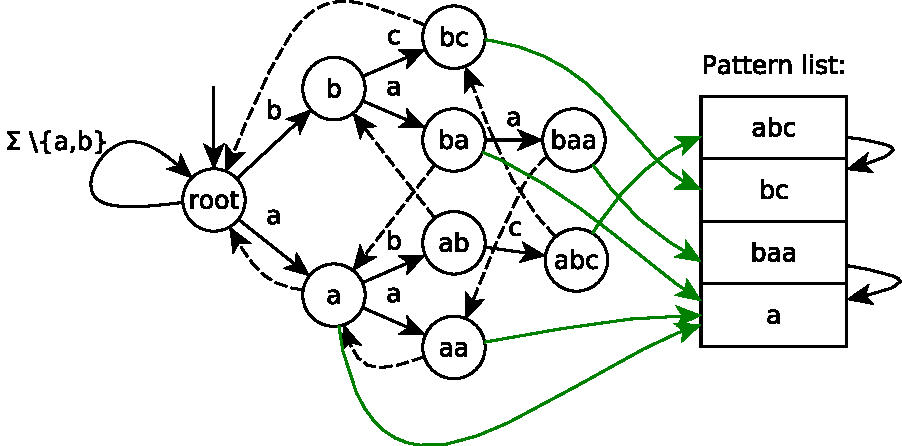
\includegraphics[width=23cm]{aho_corasick.pdf}
\caption{Aho-Corasick automaton with failure links and pattern list}
\end{figure}


\section{Experiments}

The style supports all of the university's different faculties and special departments which have an official colour scheme.


\section{Conclusions}

The colour scheme of the following faculties and departments is supported. This is a comprehensive list of all the official color schemes defined for our university.

\begin{itemize}
\item Faculty of Agriculture and Forestry 
\item Faculty of Arts 
\item Faculty of Behavioural Sciences 
\item Faculty of Biological and Environmental Sciences 
\item Faculty of Law 
\item Faculty of Medicine 
\item Faculty of Pharmacy 
\item Faculty of Science 
\item Faculty of Social Sciences 
\item Faculty of Theology 
\item Faculty of Veterinary Medicine 
\item Swedish School of Social Science
\item Aleksanteri Institute
\item Center for Information Technology
\item Center for Properties and Facilities
\item Helsinki Collegium for Advanced Studies
\item Institute of Biotechnology
\item Laboratory Animal Centre
\item Language Centre
\item Neuroscience Center
\item Open University
\item Palmenia Centre for Continuing Education
\item Ruralia Institute
\item University of Helsinki Library
\item None (plain black and white)
\end{itemize}


\section{Can I help?}
There are still various issues with the style. There are some problems with math fonts which I haven't been able to solve to my satisfaction.

Contributions and comments are always welcome. Contribute on Github or send email to \url{olli.wilkman@iki.fi}.


\newcolumn

\section{Example 1: math}
You can more or less use all the nice math features of \LaTeX~in your poster:

\begin{equation}
	\int_{-\infty}^{\infty} \frac{1}{\sqrt{2 \pi \sigma^2}} \exp\left(-\frac{(x - \mu)^2}{2 \sigma^2} \right) dx = 1
\end{equation}

\begin{equation}
	P(x) = \left\{ \begin{array}{lr} \frac{1}{6}x(x-1)&,\; 0 \leq x \leq 1 \\ 0, & \text{otherwise}  \end{array} \right.
\end{equation}

\begin{equation}
	\sum_{n=0}^\infty \frac{1}{2^n} = 2
\end{equation}



\section{Example 2: Images and References}
Including images is simple.  With pdf\LaTeX, you can use images in many common formats, including PNG and JPEG, though in a poster you should strive to use scaleable graphics, for example in PDF format. Due to a limitation of pdf\LaTeX, EPS graphics do not work, but they can be converted to PDF.
	
Using labels to refer to figures and tables also works like it should, as demonstrated by these references to Figure \ref{examplefigure} and Table \ref{tableexample}.

\begin{figure}
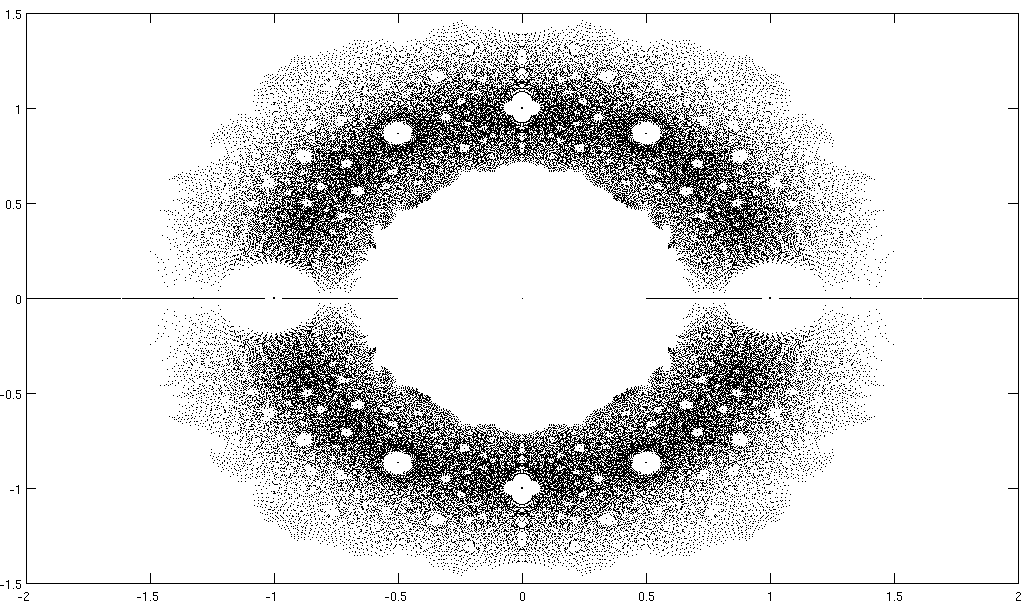
\includegraphics[width=0.8\textwidth]{zeros.png}
\label{examplefigure}
\caption{Some mathematical plot}
\end{figure}

Image courtesy of Janne Korhonen.


\section{Example 3: Tabulated table}

Table environments work, too.

\begin{table}
	\begin{tabular*}{0.5\textwidth}{@{\extracolsep{\fill}} c|r|r|r }
		$x$ & $x^2$ & $x^3$ & $x^4$\\
		\hline
		1 &  1 &   1 &   1 \\
		2 &  4 &   8 &  16 \\
		3 &  9 &  27 &  81 \\
		4 & 16 &  64 & 256 \\
		5 & 25 & 125 & 625 \\
	\end{tabular*}
	\caption{Some natural numbers and their first few powers.\label{tableexample}}
\end{table}

\section{Where can I find it?}
HYposter is hosted at Github for ease of development and cooperation. Get it at \url{https://github.com/dronir/HYposter}.


\end{poster}
\end{document}
